%%%%%%%%%%%%%%%%%%%%%%%%%%%%%%%%%%%%%%%%%%%%%%%%%%%%%%%%%%%%%%%%%%%%%%%%%%%%%%%
%% Structural analysis of IrO2 and IrO3 oxides
%% NOTES:
%%   - Describe convex hull, classes of structures (\ce{$\alpha$-AlF3} like, rutile like, and layered, should be segregated in hull plot)
%%   - Briefly describe structures within each class, cite in literature where appropriate
%%%%%%%%%%%%%%%%%%%%%%%%%%%%%%%%%%%%%%%%%%%%%%%%%%%%%%%%%%%%%%%%%%%%%%%%%%%%%%%


% ################################# Paragraph #################################
% %%%%%%%%%%%%%%%%%%%%%%%%%%%%%%%%%%%%%%%%%%%%%%%%%%%%%%%%%%%%%%%%%%%%%%%%%%%%%
% TEMP
% %%%%%%%%%%%%%%%%%%%%%%%%%%%%%%%%%%%%%%%%%%%%%%%%%%%%%%%%%%%%%%%%%%%%%%%%%%%%%
% | - Paragraph start
Here we describe the structural variety that is present in our data set of ~1000 IrO2 and IrO3 polymorphs.
% Looks like I wasn't using the algorithm implemented in R52 (David Waroquiers)
The coordination environment package ChemEnv,
developed by Waroquiers et. al. \cite{Waroquiers2017} and implemented in pymatgen \cite{Ong2013},
was used to assign the coordination motiff types (e.g. octahedral, square pyramidal, cubic, etc.) to each of the ~1000 structures in our IrOx data set.
%
Additional esoteric coordination environments were identified manually, see SI.
% COMBAK What normalization methodd do I end up using for the E and V?
The resulting distribution is included in figure TEMP, which plots the electronic energy and volume, both normalized on a per atom basis
% __|


% | - Figure | Energy vs Volume (motiff distribution)
\begin{figure*}
\centering
\makebox[\textwidth][c]{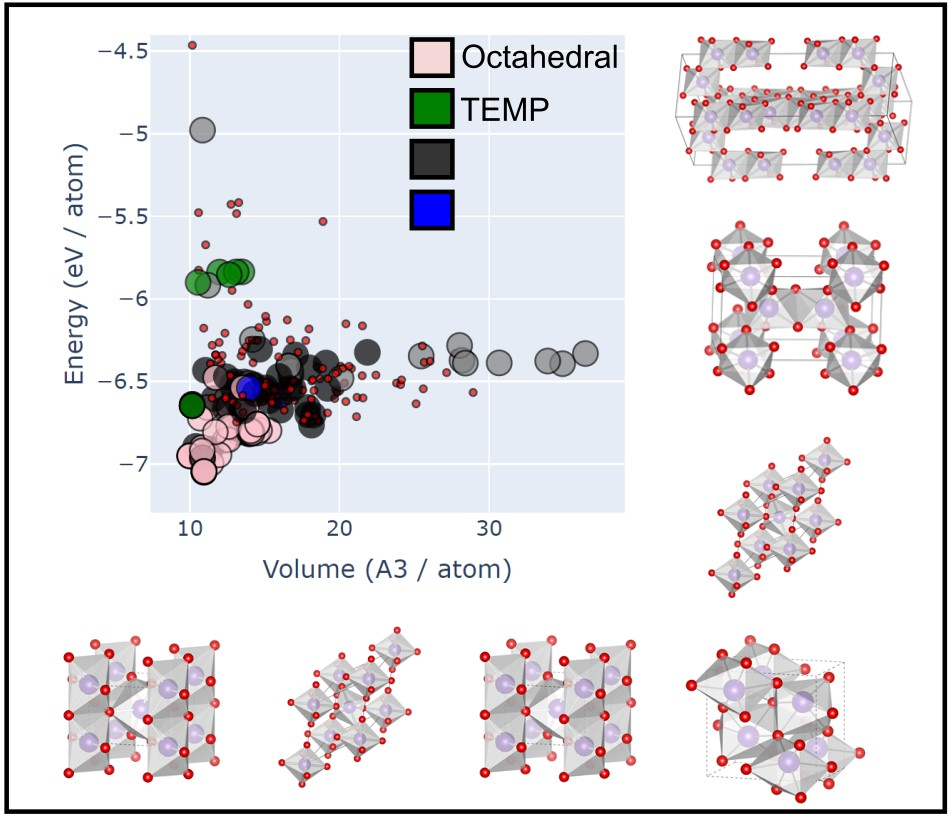
\includegraphics[
width=\textwidth,height=\textheight,keepaspectratio]
{02_figures/e_vs_v_motiffs.jpg}
}
\caption{\label{fig:iro2_al}
% Make sure to update x-axis quantity (volume per atom, Ir, or density, etc.)
Enthalpy of formation for the TEMP|num-iro2-dft IrO2 (circles) and TEMP|num-iro3-dft IrO3 (crosses) structures in the candidate data set plotted against the volume per atom.
%
Color overlays indicate the dominant coordination motiffs as indicated by the legend.
%
Select polymorphs systems are displayed around the plot area.
}
\end{figure*}
% __|






% | - __old__

% | - Figure | IrO2 Convergence Plot
% \begin{figure*}
% \centering
% \makebox[\textwidth][c]{\includegraphics
%   {02_figures/ml_convergence_plots/00_master__iro2-ml-conv_v1__200dpi__0__outplot.png}
%   % {02_figures/ml_convergence_plots/iro2_ml_conv.png}
%   }
% \caption{\label{fig:convergence_plot_iro2_0}
% % #COMBAK Subscript IrO2
% Gaussian process machine learning models trained initially on (a) publicly available DFT data for IrO2 and (b) all of the acquired DFT calculations from the active learning algorithm.
% See SI for additional panels at intermediate iterations of the active learning algorithm.
% The Gibbs formation energy (either DFT derived or predicted from the GP model) and associated GP estimated error (2 sigmas or something TEMP) is plotted for each polymorph in the IrO2 candidate space.
% The data points in each subset are ordered from most to least stable (lowest to largest DE formation).
% The individual markers are colored based on their ordering in the final converged GP model.
% Acquired structures are identified by their red borders and slightly larger size.
% The insets show the most stable TEMP structures, where several well known crystal structures are labeled.
% }
% \end{figure*}
% __|

% | - Figure | IrO3 Convergence Plot
% \begin{figure*}
% \centering
% \makebox[\textwidth][c]{\includegraphics
% {02_figures/ml_convergence_plots/00_master__iro3-ml-conv_v6__200dpi__0__outplot.png}
% % {02_figures/ml_convergence_plots/iro3_ml_conv.png}
% }
% \caption{\label{fig:convergence_plot_iro3_0}
% TEMP.
% }
% \end{figure*}
% __|

% __|
